\section{Procedure}
\label{sec:procedure}
The following part describes the experimental set up and procedure. It is based on the given
instructions and has been modified to the actual procedure in the lab.

\subsection{Measuring the speed of light through phase differences}
\label{sec:measuring}
\begin{figure*}
    \centering
    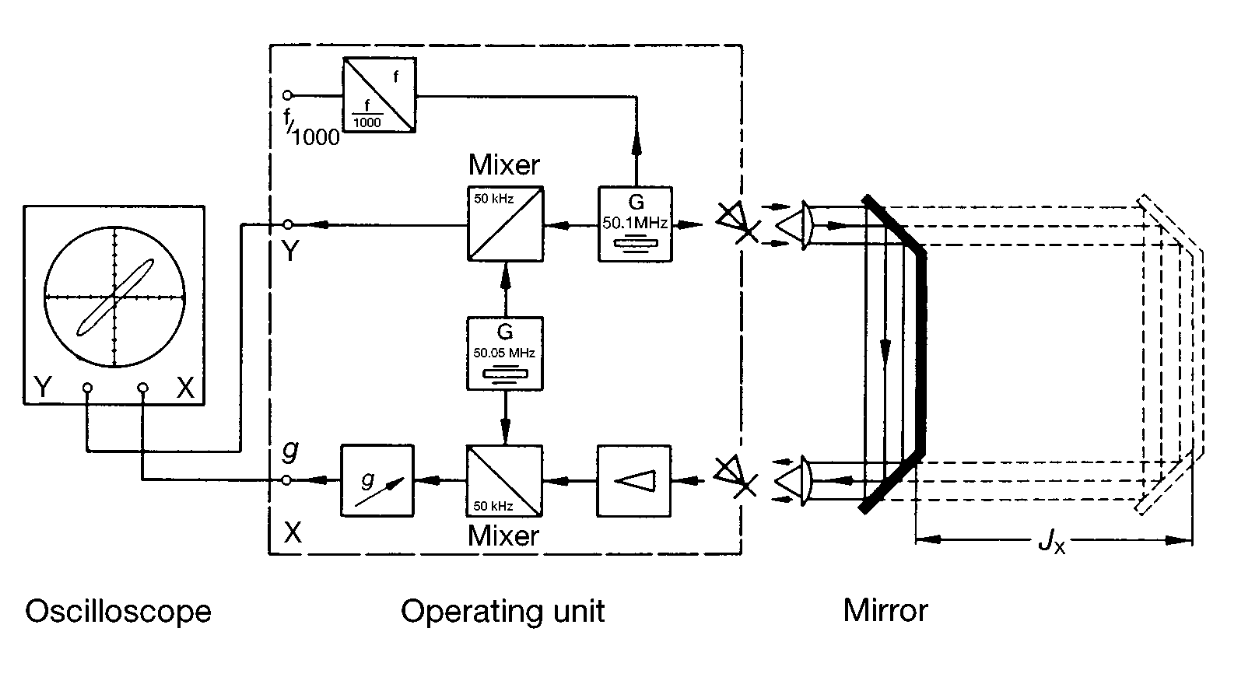
\includegraphics[width=0.8\textwidth]{media/Setup Air.png}
    \caption{Diagram of the experimental set-up for measuring the velocity of light in air. Taken
      from the instructions given for this experiment \cite{LabInstructions}.}
    \label{fig:SetupAir}
\end{figure*}
To measure the speed of light in air, a setup as shown in \autoref{fig:SetupAir} is used. A source
is sending a pulse of modulated light towards a mirror setup where it gets
reflected to the detector unit. An oscilloscope attached to the operating unit shows a Lissajous
figure corresponing to the phase difference between sent light and received signal.

For each measurement, the distance between the mirror and operating unit gets extended by
\[
\Delta x,
\]
resulting in an extra light path
\[
  \Delta l = 2 \Delta x.
\]
$\Delta x$ is chosen such that a phase change of $\pi / 2$ is added. The originally intended $\pi$
were not possible as the light source lost its definition after $\Delta x \gtrapprox \SI{1}{m}$.

To travel the distance $\Delta l$, light needs the time
\[
  \Delta t = \frac{1}{4f}
\]
with the \textit{modulation frequency} $f = \SI{50.1}{MHz}$. Since
\[
  \text{Speed} = \frac{\text{Distance}}{\text{Time}},
\]
we can conclude that
\begin{equation}
  c = \frac{\Delta l}{\Delta t} = 8f \Delta x.
  \label{eqn:speedoflight}
\end{equation}

\subsection{Measuring the speed of light in resin}
\label{sec:MeasuringResin}
To measure the speed of light in resin $c_M$, the same operating unit as in \autoref{sec:measuring} is
used. This time however, a block of synthetic resin of length $l_M$ is put in one ligth beam between
operating unit and mirror.

Afterwards, the block gets removed and the distance between the mirror and operating unit gets
increased by $\Delta x$, such that the phase is the same as it was in the first step.

From these two steps we can compute the speed of light in resin by seeing that for the first step
\begin{align}
  l_1 &= 2 x_1 \\
  t_1 &= \frac{1}{c_\text{Air}} (l_1 - l_M) + \frac{l_M}{c_M}
\end{align}
and in the second step the distance and time difference are
\begin{align}
  l_2 &= l_1 + 2\Delta x \\
  t_2 &= \frac{1}{c_\text{Air}} (l_1 + 2 \Delta x).
\end{align}
In these expressions the speed of light in air $c_\text{Air}$ is assumed to be known. For the calculation
we
use the result from \autoref{sec:measuring} as a speed of ligth in air.

Since in both cases the phase is the same, the travel times have to fulfill 
\[
  t_1 = t_2 + \frac{k}{f}
\]
with $k\in\mathbb{N}$. One can rearrange the equations to obtain the refractive index
\begin{equation}
  n = 1 + \frac{2 \Delta x}{l_M} + \frac{k c_\text{Air}}{f l_M}.
\end{equation}
The speed of light in resin can then be computed with the formula
\begin{equation}
  c_M = \frac{c_\text{Air}}{n}.
\end{equation}

\begin{figure}
    \centering
    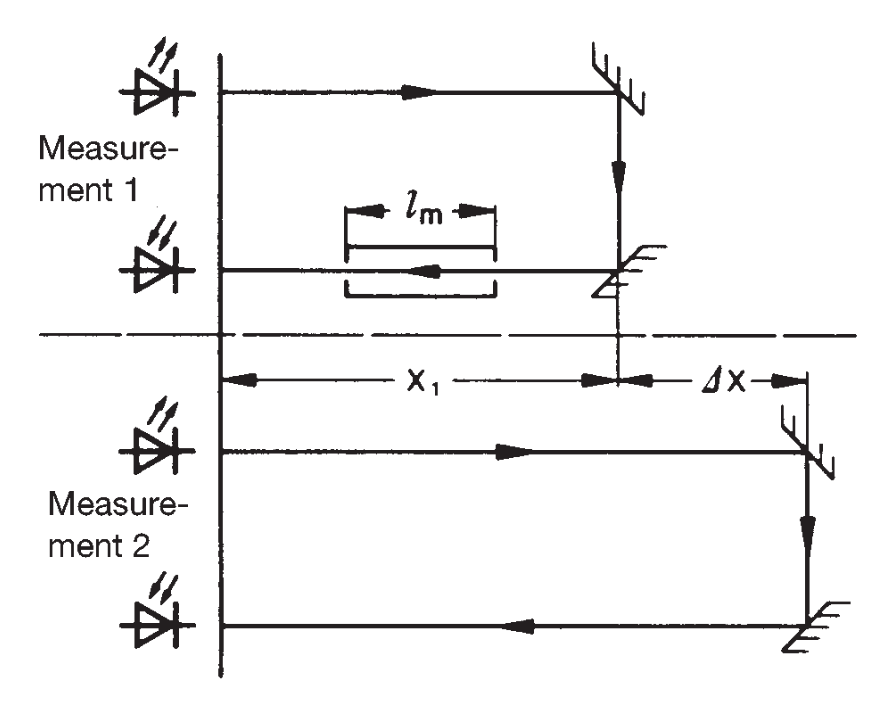
\includegraphics[width=0.4\textwidth]{media/Setup Resin.png}
    \caption{Measuring the velocity of light in other media. Taken
      from the instructions given for this experiment \cite{LabInstructions}.}
    \label{fig:SetupResin}
\end{figure}

